\chapter{Introduction}
\label{Chapter:Introduction}
The world is working to move away from fossil fuel as its main energy source \cite{ValluriPHD}. \acf{nrel} has partnered with over 700 organizations, including large manufacturing companies, to de-carbonize supply chains \cite{NREL-partner}. Nuclear power has been well established as an alternative for base-load electrical generation with 93 facilities in the United States and 435 globally which generate on the order of 1 GWe, but there remains a need for smaller reactors to be deployed in more dynamic applications such as small remote grids (including military bases \cite{AirForce}), manufacturing, and power-peaking \cite{DoD-remote}. These small energy utilizers could turn to microreactors to fill their needs; to make this a reality, a robust control system for microreactors must be designed that is capable of ramping production up and down to meet demand.

\section{Microreactors}
Microreactors, as the name suggests, are small nuclear reactors which are designed to be fully assembled when shipped, rather than constructed on site. This is a hot area of research in the private sector as companies are working to capitalize on the growing need for clean and dependable small scale electrical generation \cite{PetersonMS}. They aim not to replace the utility scale \acfp{npp} which handle base-load electrical generation, but the diesel or natural gas engines that are found at countless manufacturing facilities, peaking stations, military bases, islands, and other locations where on-site generation is the primary or only source of electricity. 

The goal is to be able to deliver a prefabricated microreactor to a site, integrate it to the necessary power cycles and process heat applications, and meet the needs of the site for a long period of time - up to a decade - without the need for refueling or significant maintenance. This would be quite convenient compared to building a pipeline to deliver fossil fuels to the site or scheduling regular delivery. One of the biggest challenges in implementing microreactors is the transients that these applications often require. Engines handle these quite well, simply adjusting the flow rates of fuel and combustion air. Nuclear reactor load following is a bit more complicated, as the reactor must be made supercritical to ramp up power or subcritical to decrease power. This necessitates valid characterization of the reactor's criticality control \& actuation system and reactivity feedback mechanisms, so an effective `reactor-following-turbine' controller can be tuned \cite[Ch. 8]{Kerlin}.

\section{\texorpdfstring{\aclp{msr}}{Molten Salt Reactors}}
Molten salts are highly desirable in high temperature applications due to their excellent thermophysical properties \cite{RoperReview}. Salt mixtures have been developed to have very wide liquid temperature ranges (i.e. low melting point and high vaporization point). They also have very high volumetric heat capacities compared to other high temperature coolants (which tend to be gaseous), and are able to operate at or slightly above ambient pressure. These properties combine to make molten salts excellent choices in heat transfer and thermal storage applications. Furthermore, they are extremely strong electrolytes which cn be useful as solvents, catalysts, or reagents in certain chemical reactions including a pyrometallurgical method for reprocessing spent nuclear fuel \cite{Simpson}.

\acfp{msr} are a family of nuclear reactor in which a fuel salt (containing fissile and/or fertile nuclides) is dissolved in a coolant salt \cite{RoperOverview}. The concept was proven by the \acf{msre} at \acf{oak} in the 1960s \cite{MSRE}. It has yet to take off beyond the research reactor sector, but it has re-emerged as a Gen-IV reactor concept, with a team at the Shanghai Institute of Applied Physics gaining approval to operate a now fully constructed thorium breeding \acs{msr} \cite{china}. Some of the benefits of \acsp{msr} over more conventional \acsp{lwr} include:
\begin{itemize}
    \item Higher operating temperatures allow for use in applications requiring high-grade process heat, and yield higher thermal efficiency \cite{RoperOverview};
    \item Lower pressure operating pressure lends itself to inherent safety, and less expensive (thinner) components \cite{RoperReview};
    \item The ability to burn minor actinides supports the goal of reducing global stockpiles of high-level waste \cite{RoperReview};
    \item Natural circulation of the fuel introduces an additional feedback mechanism that presents the possibility of autonomous load following of certain power demand transients \cite{CarterNumerical};
    \item There is no concern of core melt-down as the reactor is designed for liquid fuel;
    \item The liquid state homogenizes nuclides throughout the core, which minimizes burn-up gradient to produce a flatter temperature and power profile within the core \cite[Ch. 3]{TodreasKazimi1}. The flowing nature also allows for online reprocessing, removing fission products and poisons during operation;
\end{itemize}

They also carry some demerits:
\begin{itemize}
    \item Molten salts are very corrosive \cite{RoperRedox};
    \item The chemistry of the coolant (not only the fuel) is constantly changing due to fission, transmutation, and impurities from corrosion;
    \item Lithium is commonplace in molten salts, so tritium production is unavoidable (\ref{rxn:tritium}). Off-gas systems need to be robust to handle tritium as well as radionuclide noble gasses, halides, and inter-halides \cite{HolcombOffgas};
\end{itemize}

\begin{reaction} \label{rxn:tritium}
    ^{6}Li + n \to {^{3}H} + \alpha
\end{reaction}

\section{\texorpdfstring{\acl{msnb}}{Molten Salt Nuclear Battery}}
The \acf{msnb} is a self contained design for a liquid fueled molten salt microreactor \cite{CarterPHD,PetersonMS}. It is fueled by an inorganic form of uranium, \UF, dissolved in a coolant salt such as \flinak (a eutectic mixture of three alkali fluorides) or \flibe  (a mixture of $LiF$ and $BeF_2$) \cite{RoperOverview}. Heat is generated in the core by fission and is rejected in an integrated heat exchanger (Fig. \ref{fig:tikz_msnb}). Criticality is manipulated using axial control drums, which may be rotated to aim either a neutron reflecting material or a neutron absorbing material towards the core. The design studied in this work is intended to produce up to 1 MWth, although larger designs of up to 50 MWth also exist.

\begin{figure}[!ht]
    \centering
    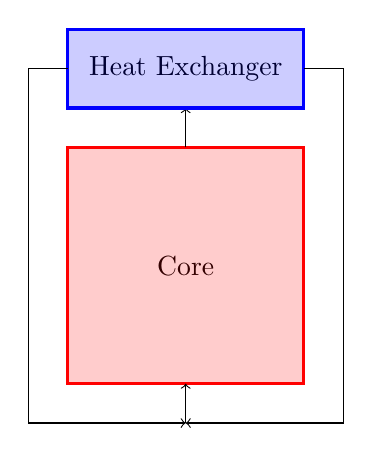
\begin{tikzpicture}
    %Core
    \draw node at (1.5,1.5) {Core};
    \draw[red, very thick] (0,0) rectangle (3,3);
    \filldraw[red,opacity=0.2] (0,0) rectangle (3,3) ;
    %Riser/Chimney
    \draw[->] (1.5,3) -- (1.5,3.5);
    %HEX
    \draw node at (1.5,4) {Heat Exchanger};
    \draw[blue, very thick] (0,3.5) rectangle (3,4.5);
    \filldraw[blue,opacity=0.2] (0,3.5) rectangle (3,4.5) ;
    %Downcomer
    \draw[->] (3,4) -- (3.5,4) -- (3.5,-0.5)  -- (1.5,-0.5);
    \draw[->] (0,4) -- (-0.5,4) -- (-0.5,-0.5)  -- (1.5,-0.5);
    \draw[->] (1.5,-0.5) -- (1.5,0);
\end{tikzpicture}

    \caption[Simplified schematic drawing of an \acs{msnb}]{Simplified schematic drawing of an \acs{msnb}. Heat is generated in the core by fission, is transported by natural circulation of the coolant/fuel salt, and rejected to a secondary working fluid in the heat exchanger before returning to the inlet plenum through the downcomer.}
    \label{fig:tikz_msnb}
\end{figure}

\section{Scope}
As a developing design, work has been done on neutronics \cite{PetersonMS}, thermal-hydraulics and autonomous load following \cite{CarterPHD}, and corrosion concerns \cite{RoperPHD}. However, until now, little to no work has been done on the control system. First and foremost, this work details a multiphysics characterization of the \acs{msnb} required to design a feedback controller capable of matching the core power generation to the secondary power demand. In addition to the main control mode of following power transients during normal operation, specific discussion is centered around more dynamic time periods, namely: 
\begin{enumerate*}
    \item initial start-up;
    \item shutdown, both planned and emergency; and
    \item restart;
\end{enumerate*}

\begin{comment}
\section{Outline}
This report will begin by discussing the field of process control engineering, specifically the control methods which are most useful in the design of a controller for the \acs{msnb}, and the challenges inherent to a controlling a nuclear chain reaction, both in normal operational modes and special cases. The reactor will then be characterized, using a combination of stochastic neutron transport code to define the reactivity curve of the control drums and finite element process simulation to understand the reactivity feedback effects intrinsic to the design. The resulting model of the reactor will then be used to design and tune the controller, which will then be tested against the reactor's autonomous response to load demand changes. Finally, after the results of the simulation are analyzed, the limitations of this method, as well as future work that will be required to implement a \acl{msnb} will be discussed.   
\end{comment}